\documentclass{paper}

\usepackage{graphicx}
\usepackage[utf8]{inputenc}
\usepackage{csquotes, ellipsis}
\usepackage[margin=3cm]{geometry}

% Information for title page
\title{Documentation for Interactive Learning Management System}
\subtitle{CS 377 Course Project}
\author{Juhao ``Jerry'' Zhang}
\institution{Emory University}


\begin{document}
	
	\maketitle
	
	
	\section{Introduction}
	
	Amazing, introductory ideas that provide unique insight into your field of interest and ``wows" your professor---formatted based on Kate L. Turabian's \emph{A Manual for Writers of Research Papers, Theses, and Dissertations} (9th edition).
	
	\section{ER Design}
	
	The following assumptions are made:
	\begin{itemize}
		\item A class must contain at least one student.
		\item A class can only be taught by one professor.
		\item A thread does not contain ``reply-to-posts'', i.e., threads will organized only by chronological order
	\end{itemize}
	The entity-relation design diagram is as follows:\\
	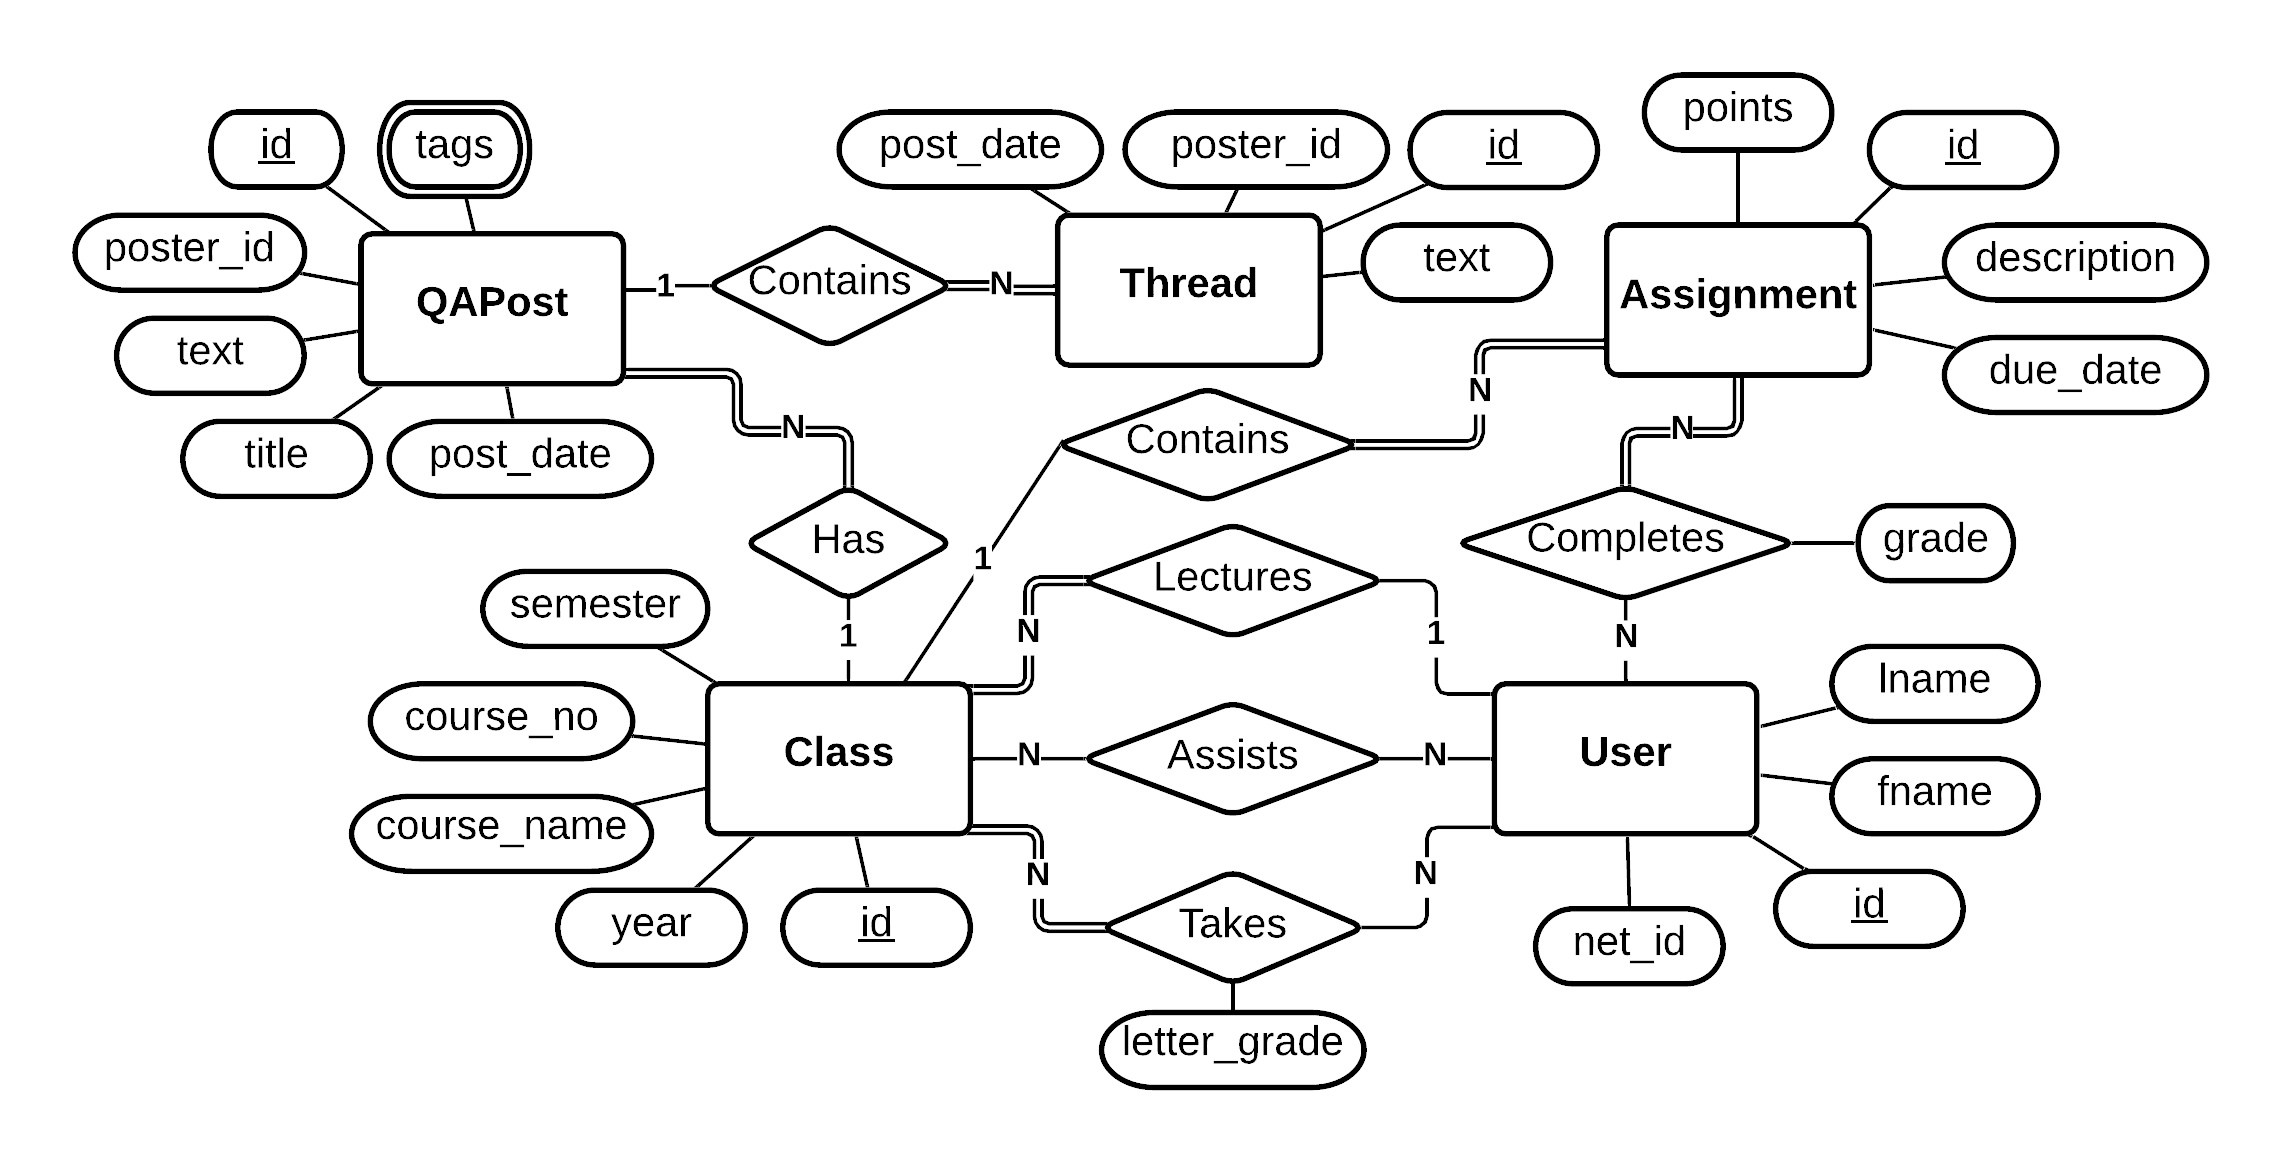
\includegraphics[scale=0.2]{er_diagram.png}

	
	\section{Relational Model Creation}
	
	The initial relational model consists of the following relations:
	\begin{itemize}
		\item User(\underline{id}, net\_id, fname, lname)
		\item Class(\underline{id}, course\_no, course\_name, semester, year, lecturer\_id$\to$User.id)
		\item Assignment(\underline{id}, description, due\_date, points, class\_id$\to$Class.id)
		\item QAPost(\underline{id}, title, text, poster\_id$\to$User.id, post\_date, class\_id$\to$Class.id)
		\item Thread(\underline{id}, text, poster\_id$\to$User.id, post\_date, parent\_id$\to$QAPost.id)
		\item Tags(\underline{post\_id}$\to$QAPost.id, tag)
		\item Takes(\underline{user\_id}$\to$User.id, \underline{class\_id}$\to$Class.id, letter\_grade)
		\item Completes(\underline{user\_id}$\to$User.id, \underline{assignment\_id}$\to$Assignment.id, grade)
		\item Assists(\underline{user\_id}$\to$User.id, \underline{class\_id}$\to$Class.id)
	\end{itemize}
	
	\section{Database Normalization}
	To ensure that the database conforms to 3NF, start by ensuring that the relation schema is in 1NF, which states that
	\begin{itemize}
		\item Every attribute in the relational model has atomic values.
	\end{itemize}
	By this rule, the relation schema is already in 1NF. 2NF states that
	\begin{itemize}
		\item 1NF is satisfied, and
		\item Non-candidate-key attributes are not partially dependent on any key of the relation, i.e., every non-key attribute is fully functionally dependent on the primary key.
	\end{itemize}
	Since the relation schema is already in 1NF, I argue the second point of the 2NF constraints: none of the non-key attributes are partially dependent on their respective relation's primary key. This can be seen readily where the primary key is a single element, and for those relations that contain a key with  size greater than 1, there are only one or no non-key attribute.\\\\
	Now, to convert to 3NF, its constraints must include that
	\begin{itemize}
		\item 2NF is satisfied, and
		\item Every non-key attribute is non-transitively dependent on all the keys.
	\end{itemize}
	I argue that the relational model proposed above satisfies the 3NF conditions, as no non-key attribute in any of the relations is dependent on another non-key attribute in that same relation.\\\\
	With the satisfaction of 3NF conditions, the normalization of the database is considered complete.
	
	\section{Data Description}
	All of the \verb|.csv| files are generated using the \verb|extract.py| script on the data source files \verb|canvas.csv| and \verb|qa.csv|.
	
	\section{PHP File Directory}
	
	\section{Conclusion}
	
	\clearpage
	
\end{document}